\subsection{Robot Design}\label{subsec:robot-design}
For this project, we elected to use a flying Tello drone.
We chose a flying drone primarily to allow the robot to get close enough to appl

\begin{figure}[htbp]
    \fontsize{7}{5}\selectfont
    \centering
    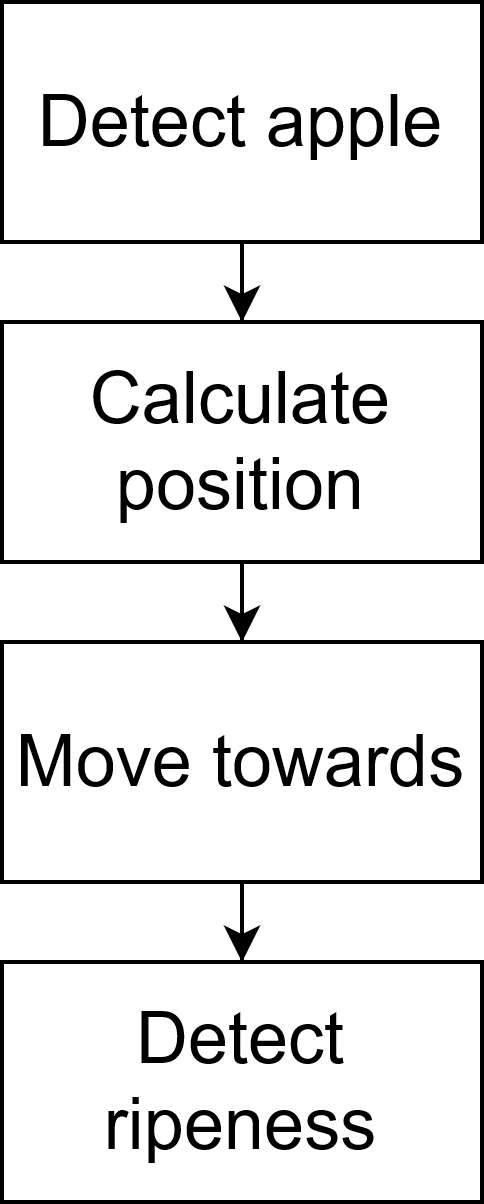
\includegraphics[maxwidth=\columnwidth,scale=0.8]
    {./figures/intelligence-hierarchy}
    \caption{
        The intelligence hierarchy used by the drone.
        Each layer is designed to minimize the work done by the controller so it does not perform expensive calculations except when needed.
    }
    \label{fig:intelligence-hierarchy}
\end{figure}

\begin{figure}[htbp]
    \fontsize{7}{5}\selectfont
    \centering
    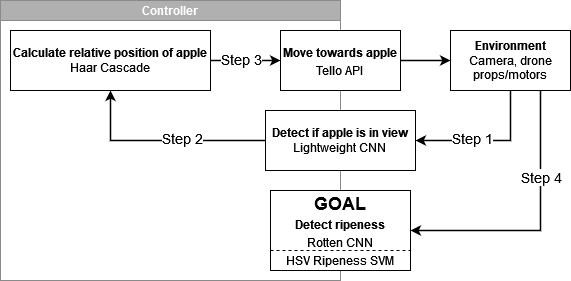
\includegraphics[width=\columnwidth,keepaspectratio]
    {./figures/fruit-fly-model-diagram}
    \caption{
        A data flow diagram of how the intelligence hierarchy works.
        The controller, which operates on another machine receives input from the drone's cameras and other sensors.
        This information is passed to a lightweight model, then to heavier models to operate the drone and determine fruit ripeness.
    }
    \label{fig:fruit-fly-model-diagram}
\end{figure}
